
%Platform developers may discover policy-violations
%through customer complaints, integration tests, or by periodically running
%invariant checks on a deployed network.

Before presenting our approach, we describe an example bug in the Floodlight
open source control platform~\cite{floodlight}. Floodlight is distributed across
multiple controllers for high availability, and provides support for
virtualization. Switches maintain one hot connection to a master controller and
several cold connections to replica controllers. The \emph{master} holds the
authority to issue state changing requests to the switches. The other
controllers are in \emph{slave} mode and do not perform any state-changes on the
switch unless they detect that the master has crashed.

\begin{figure}[t]
    %\hspace{-10pt}
    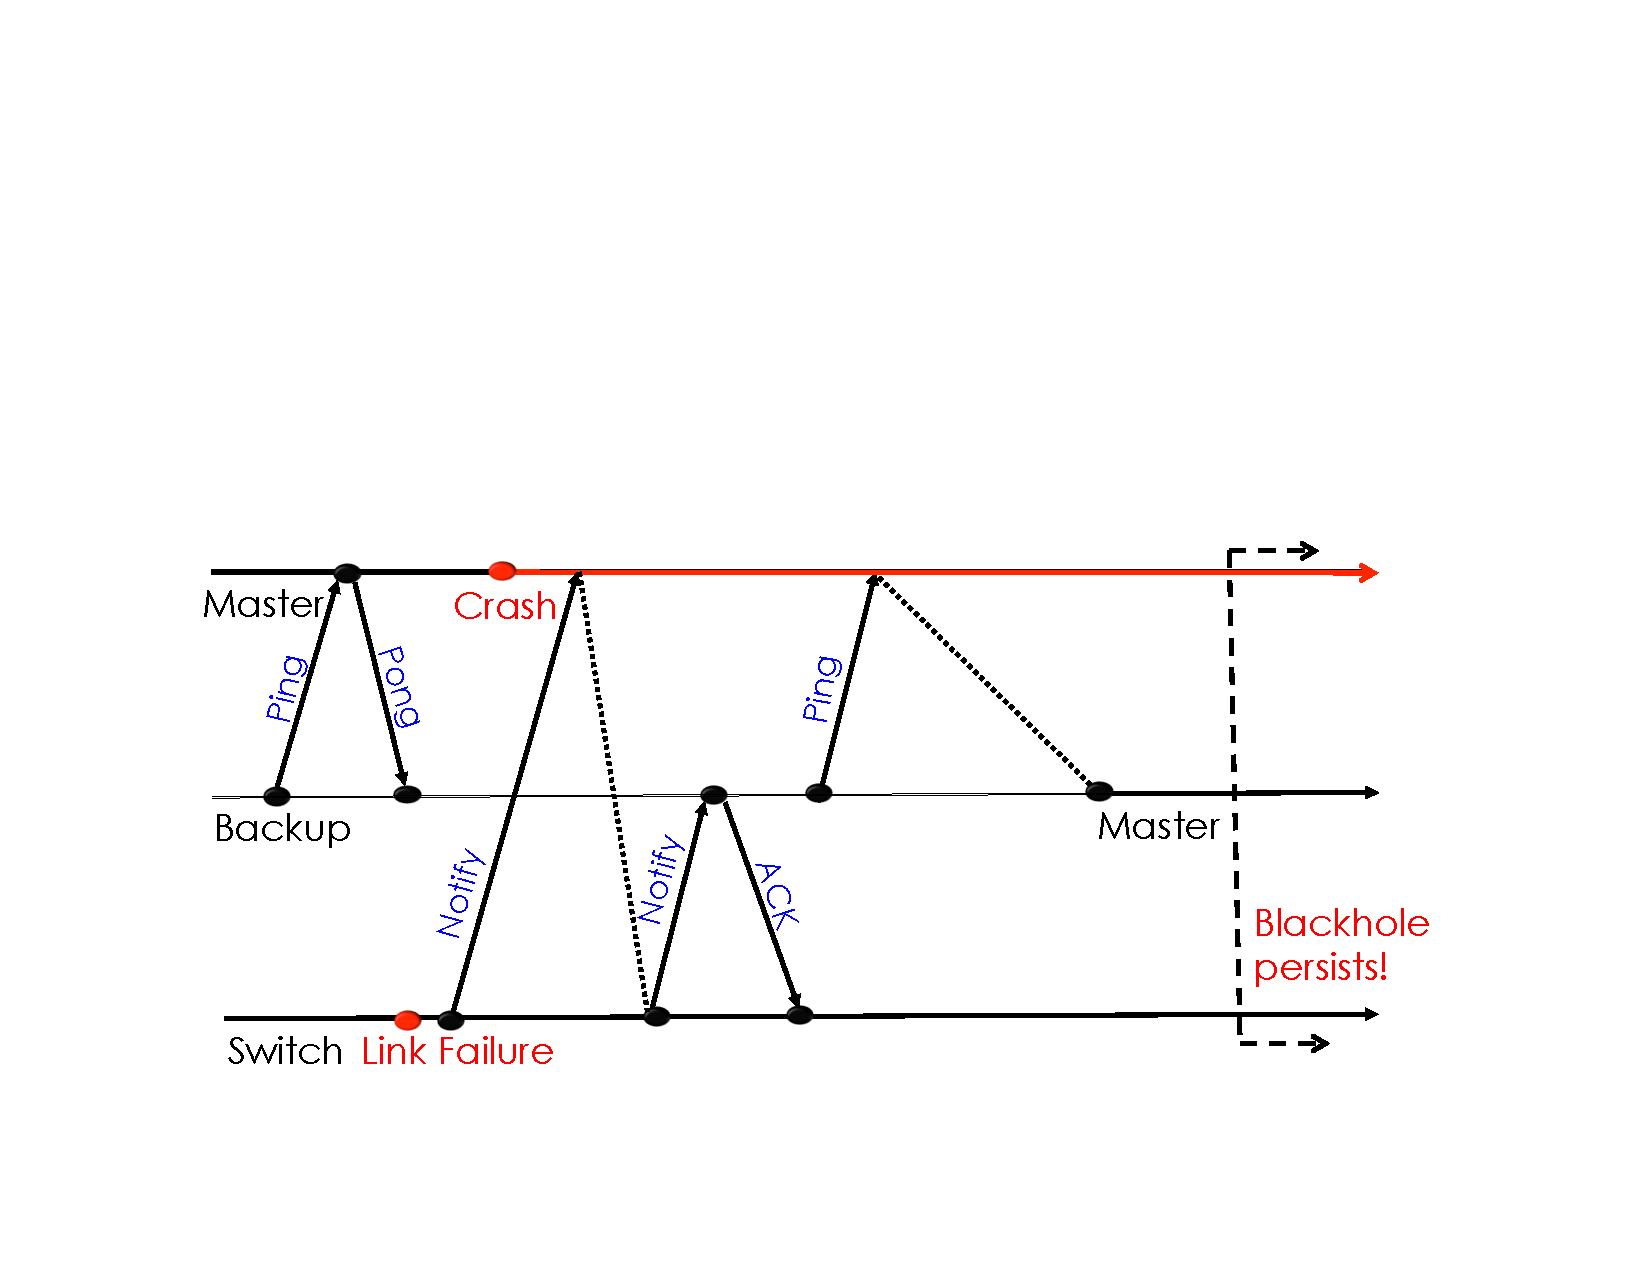
\includegraphics[width=3.25in]{../diagrams/case_study/example_bug.pdf}
    \caption[]{\label{fig:example} Floodlight failover bug. External inputs
               are depicted as red dots, internal events are depicted as black
               dots, and timeouts are depicted as dotted messages lines.}
\end{figure}

Consider the following race condition\footnote{Note that this issue was
independently discovered by the developers of Floodlight.} depicted in
Figure~\ref{fig:example}:
a link fails (E1), and the switch attempts to notify the controllers (E2,E4) shortly after the master
controller has died (E3), but before a new master has been selected (E6). In this case, all live controllers are in
the slave role and thus will not take responsibility for updating the switch
flow table (E5). At some point, the heartbeats time out and one of the controllers
elevates itself to the master role (E6). The new master will proceed to manage
the newly connected switch, but without ever clearing the routing entries for
the failed link (resulting in a blackhole).

\subsection{\SIMULATOR{}}
\label{sec:causal_analysis}

Given a log of the system execution similar to the Floodlight case,
our goal is to prune events that are not
necessary for triggering errant behavior. We define errant behavior in terms of {\em policy-violations}:
configurations of the network that are inconsistent
with the policy. In the example, the policy-violation is between a
reachability policy specified in the logical view (``A can talk to B'')
and the blackhole in the physical network (``A's packets to B enter the
blackhole and do not arrive at B'').

There were only two inputs (link failure, and server crash) shown in our example.
In production datacenter logs
a significantly greater number of hardware failures, topology changes,
and other potential triggering events will be present,
all of which may appear characteristic of normal operating
conditions at first glance; assuming 8.5 network error events per
minute~\cite{Greenberg:2009:VSF:1592568.1592576}, 500 VM migrations per
hour~\cite{Soundararajan:2010:CBS:1899928.1899941}, and a relevent execution
history of one hour, there would be over 1000 extraneous inputs to the system
reflected in the log.

We have developed an algorithm, \simulator{}, for automatically inferring the inputs to the
controllers  that are both necessary and sufficient for triggering the policy-violation. We
refer to these events as the {\em minimal causal sequence} (MCS). The
algorithm itself shown here, and elaborated in later sections:

\begin{algorithmic}
\State $MCS \gets []$
\ForAll {\text{\it external input in log}}
    \State {\it remove first input from log}
    \State {\it bootstrap system}
    \State {\it rerun execution with modified input}
    \State $violation \gets detect\_violation()$
    \If {\it not violation}
        \State $MCS << event$
        \State {reinsert input to front of log}
    \EndIf
\EndFor
\end{algorithmic}

\noindent In words, the algorithm takes in a log of the system execution,
prunes each external input in isolation (assuming that inputs are causally
independent, thereby avoiding exponential runtime),
runs the system forward with the remaining input, checks whether the
policy-violation is still present, and thereby infers whether that input is
necessary for triggering the fault. Going back to our example, suppose the
log includes many more inputs (policy changes, host migrations, hardware
failures) than just the link failure and the controller crash. Whenever an
extraneous event is pruned, the blackhole will still persist. When
the controller crash is pruned, the blackhole will be resolved properly, and
when the link failure is pruned, no blackhole will occur. The MCS returned
is therefore the controller crash and the link failure in conjunction.

The crux of our problem lies in specifying exactly how each
individual step of this algorithm works. In the rest of this section we will
detail the (i) distributed logging infrastructure, (ii) deterministic
replay execution environment, and (iii) violation detection algorithms
necessary for finding the minimal causal sequence.

\subsection{Distributed Logging}

\Simulator{} first requires a log of the system execution where a
policy-violation was originally discovered. Policy-violations
in a running system might be detected through failed integration tests,
customer complaints, or runtime invariant checks.

Since our goal is to identify
relevant {\em inputs} from the distributed system's log, the log must make a clear
distinction between {\em internal} events such as control message sends and
receives, and {\em external} inputs such as
link failures, controller crashes, VM migrations, or policy changes.
Production networks almost universally maintain logs of such events as part of
good operating practices (link failures are typically detected through
protocols such as IS-IS,
controllers log crash messages before
halting in addition to monitoring heartbeats from peers, and VM migrations and
policy changes are logged centrally for accounting purposes). In case
that an input to the system is not present in the available logs,
\simulator{} may not reproduce the policy-violation, and the developer will
have to ensure that the logging messages are added to the system.

\Simulator{} also depends on a correctly ordered, `global' log of the
distributed system's execution. If the control software does not already do
so, we modify the code to attach Lamport
clocks to all
control packets and internal log messages
to achieve a total ordering of the events in the system that
is consistent with the happens-before
relation~\cite{Lamport:1978:TCO:359545.359563}. Note that it is not
strictly necessary that the log match the production execution perfectly, so
long as the policy-violation still occurs at the end of the replayed
execution.

\eat{
As an optimization, the developer may start from a causally-consistent
snapshot of the network rather than replaying the execution from the
very beginning of the log. In this case, the user would need to occasionally
execute a consistent-snapshotting algorithm~\cite{Chandy:1985:DSD:214451.214456}
on the live deployed system, and start \simulator{} from a quiescent snapshot.
}

%(ii) We assume that the causally-consistent snapshot we start from is quiescent. [it's possible that a member of the MCS occurred before the snapshot was taken]
%
%Solution/Workaround: once we've run the MCS algorithm, re-run it from an earlier snapshot and see if the MCS changed. Technically this process would have to be applied inductively, but we could parameterize the number snapshots we have to examine.
%
%Discussion: it's also not a huge deal if this assumption does not hold. The policy-violation will still be detected -- the only problem is that the MCS will be smaller than it actually is. Moreover, as the software developer starts debugging the problem, she'll eventually notice that some piece of state at the point of the snapshot is incorrect, and therefore she'll notice that she needs to start from an earlier snapshot.

\eat{
\colin{In the simulator, this consistent snapshot is
trivial to take: simply pause each controller's VM and the simulation. To
obtain the snapshot that denotes time zero, we assume that the production
network takes periodic snapshots using an algorithm such as Chandy et al's
\cite{Chandy:1985:DSD:214451.214456} consistent snapshot algorithm}
}

\eat{
{\em Causally-consistent snapshot:} a snapshot of a distributed system's state where
there exists no event $b$ in a node's event history such that $a \rightarrow
b$, but $a$ does not appear in the snapshot.
}

\eat{
{\em External events:} input fed to the control platform triggered by processes outside
of the system. For proactive controllers, external input includes policy
changes, host placement changes, network topology changes (including hardware
failures), and control server failures. Reactive controllers
additionally take traffic changes as input. External events are to be distinguished
from internal events triggered by the system itself, such as message sends or software
crashes.
}

\subsection{Deterministic Replay}

Next, \simulator{} requires the ability to replay the system execution.
We have developed solutions to two separate challenges in achieving this requirement.

First, the system replay has to be {\em deterministic}.
We achieve this with a single-threaded simulator that models switches
and hosts in the network. We run the controllers in individual VMs that are
bootstrapped from a static snapshot (including random number generator
seeds, \etc{}) and connect the simulated switches to the controllers as if they were true
network devices. The simulator interposes on all communication channels in
the network, allowing it to proceed with the system execution in lock step:
pausing the controller VMs between each logical timestep and delaying messages
arbitrarily. The simulator then reproduces the external inputs from the log.
For example, link failures are reproduced by disconnecting the edge in
the simulated network. The simulator can replay policy-changes by
interfacing through generic interfaces to SDN control platforms such as the
Quantum API~\cite{quantum}.

Note that the simulator does not need
to precisely reproduce the failure modes of {\em individual} nodes.
We are only interested in observing the behavior of the overall distributed system, which is
built under the assumption that individual components will fail.
Therefore, it is sufficient to use a `blunt hammer' (\eg{}
$kill \text{ -}9$) to reproduce individual
failure events, so long as the remaining nodes in the system react in the same
way as they did in the actual run.

Second, we need to know precisely {\em when} to inject inputs to the controllers;
without maintaining the exact happens-before dependencies reflected in the
log the output of the simulated system execution may not be the same.

We can inject an external input $e$ at exactly the point where all other
events (both external and internal) that precede it in the happens-before
relation ($\{i \mid i \rightarrow e\}$) have occurred. Unfortunately the problem is made
substantially more complicated by the fact that we are pruning inputs to the
system, thereby changing the resulting internal events generated by the control
software; without knowing in advance what internal events will {\em not} occur
as a result of pruning an external input, we can never know when the happens-before
dependencies have
been met. We solve this problem by modifying the control software to include causal
annotations~\cite{xtrace} on all log and control messages, yielding a tree of
causal offspring for any given event. When we prune an input $e$, we then remove
all of its causal offspring from the set of
happens-before constraints. Modifying the control software incidentally solves two
additional problems: the simulator can know exactly when internal controller events
occur since we can interpose on the causal annotation library, and
the simulator can infer equivalent internal events between runs despite minor
syntactic differences (\eg{} sequence numbers on packets) by
uniquely identifying events according to their place in the causal call graph.

%\colin{
%Note that in the absence of causal annotations it is still feasible to replay
%the system execution by naively injecting inputs using timers, although the
%output of the algorithm is not guaranteed to be exactly correct.
%}

\subsection{Correspondence Checking}

Finally, we need a mechanism for deciding
whether a policy-violation is present at the end of the system execution.
We refer to such an algorithm as a {\em decider}. Deciders take as input a
causally-consistent snapshot of the system state, and return whether the
policy-violation they were designed to detect is present.

We develop a particular decider here, which we refer to as correspondence checking.
Correspondence checking is generic, in the sense that it does not require
the user to specify invariants. Instead, correspondence checking returns a list
of policy-violations present in the network, and the user checks whether the
policy-violation in mind is present in the list.

In short, correspondence checking provides a crisp determination of all possible packet inputs that
would not behave according to the application's policies if injected into the
network. Correspondence checking builds on the virtual packet algebra pioneered in headerspace
analysis~\cite{hsa}.

\eat{Furthermore, running correspondence
checking between intermediate layers of the SDN stack (logical view versus
physical view), allow us to identify the component(s) of
the system where policy-violations first manifest themselves.}

Formally, the state of the physical network, the physical view, and the
logical view can be represented as graphs,
$G = (V, E)$. Packets are series of bits, $h \in \{0,1\}^L = H$,
where $L$ is the maximum number of bits in the header.

Upon receiving a packet,
forwarding elements apply a transformation function, potentially modifying
packets before forwarding them on\footnote{Multicast forwarding can expressed
by extending the range to sets of output tuples}:
\begin{align*}
T: (H \times E) \rightarrow (H \times E_{\emptyset})
\end{align*}
Here, $E_{\emptyset} \equiv E \cup \emptyset$, signifying that forwarding elements
may drop packets.

We use $`\Psi`$ to denote the collection of all transfer functions present in
the network at a particular point in time. In this model, network traversal is
simply repeated application of $`\Psi`$.
For example, if a header $h$ enters the network through edge
$e$, its state after $k$ hops will be:
\begin{align*}
\Psi^k(h,e) = \Psi(\Psi(\dots \Psi(h,e)\dots))
\end{align*}

The externally visible behavior of the network can be expressed as the
transitive closure of $\Psi$:
\begin{align*}
\Omega: (H \times E_{access}) \rightarrow (H \times E_{\emptyset}) \\
\Omega(h,e) = \Psi^{\infty}(h,e)
\end{align*}
Here, $E_{access}$ denotes access links adjacent to end-hosts.

The domain of $\Omega^{physical}$ is the set of pairs of end-hosts in the
physical network along with packets that they could possibly produce (before
the outgoing interface has encapsulated them). We define $\Omega^{view}$ in exactly the same way, where
the logical hosts are abstract representations of the hosts in the physical
network. This definition depends on the observation that end-hosts are represented
in all layers, even if there is not a one-to-one mapping between the
internal vertices of $G^{virtual}$ and $G^{physical}$.

The range of $\Omega$ is the hypothetical final location and state of the
input packet if it were injected in the network.
Note that packet transformations are reflected in
$\Omega$. For example, if an input packet passes through a NAT,
the source address of the associated output packet will be re-written
appropriately. We also use the special values $DROP$ and $LOOP$ to distinguish
a packet dropped by a network device from a packet entering an
infinite loop (both packet drops and loops prevent the packet from ever leaving the network).

In SDN, it should always be the case that:
\begin{align*}
\Omega^{view} \sim \Omega^{physical}
\end{align*}
The equivalence $\sim$ means that the final outcome of any input packet
injected at a host $a_{physical}$ in the physical network has the same hypothetical final outcome as
the same input injected at the corresponding $a_{logical}$, and vice versa.

Correspondence checking takes as input a causally-consistent
snapshot of both the physical network and the
controllers' state. We first modify the controller to present an
interface through which the physical and virtual views can be
extracted. In our simulated environment, the snapshot is
then obtained by pausing execution and invoking this interface.
The routing tables of forwarding elements in the views and the physical
network can then be translated into transformation functions.
Finally, we feed a symbolic packet $x^L$ to each access link of the
network.\footnote{The rules for process wildcard bits $x^n$ are defined in
the HSA paper~\cite{hsa}} The end result is a propagation graph representing
all possible paths taken by a packet injected
at the access link.

We compute $\Omega$ by traversing the resulting propagation graph. If a packet
is dropped, or enters a loop before exiting the network, we mark the value as
$DROP$ or $LOOP$. Otherwise,
the leaves of the propagation graph define the final outcomes of the input
packets injected at that access link.

Because network policies are defined by
configuring the logical view, any mismatch between $\Omega^{view}$ and $\Omega^{physical}$
represents an instance of a policy-violation.

Note that correspondence checking does not require the user
to define any invariants. Consequently, correspondence checking represents a somewhat weak notion of
correctness. Correspondence checking only captures external behavior and
loops; it does not capture internal behavior such as load-balancing
over links. It also assumes that the policies as expressed by the
configuration of the logical view are correct; a user would need to add a more
stringent invariant check to detect misspecified policies.
Finally correspondence checking can not verify
time-dependent policies such as ``No link should be congested more than 1\% of
the time'', or ``No server should receive more than 500MB/s of external traffic''.

%\subsection{Putting it all together}
%
%MCS assumptions:
%
%(xi) We assume causally independent external input
%
%Solution: Argue that we don't need to model drunk network operators
%
%(xii) We assume that the policy-violation detector algorithm can unambiguously identify violations. [Will the symptom ever be slightly different on the next iteration of the system?]
%
%Solution: HSA gives a pretty precise determination of the policy-violation
%

% --------------- Some Relevant thoughts ---------------------

%\colin{To get a better sense of the inputs to the controller, perhaps we should take
%a look at the Quantum plug-in API.}

%\colin{
%Vector clocks as an optimization for causal inference. (If concurrent,
%can prune automatically)
%}

% ============ TERMS ================
\eat{
{\em happens-before:} a transitive relation $\rightarrow$ on the external and internal events of
the system execution, following Lamport's
formulation~\cite{Lamport:1978:TCO:359545.359563}: (i) if $a$ and $b$ are
events in the same process and $a$ comes before $b$, then $a \rightarrow b$,
(ii) if $a$ is a message send by one process and $b$ is the receipt of the
same message by another process, then $a \rightarrow b$. A happens-before
relation defines a partial ordering on the events in the system execution.

Happens-before is to be distinguished by causality. happens-before says "could
have caused". Causality says "actually affected the behavior"
}

% ============ /TERMS ================


% --------------- /end Some Relevant thoughts ---------------------


% ------- Old Additional Use-Cases section -------

\eat{\subsubsection{Additional Use-Cases} Besides lifetime tracking and causal analysis, our simulation infrastructure has a

number of other possible use-cases:

\colin{Make sure we describe how the policy-violation of interested is
originally identified by the operator/developer. Also don't forget to
emphasize the distinction between transient and persistent

Correspondence checking infers all policy-violations in the network at a
particular point in time. However, troubleshooters
need two additional pieces of the diagnostic puzzle.

First, in large distributed
systems with communication delay and hardware failures, transient policy-violations
are unavoidable, even common. That is, every time there has been a link failure that the SDN platform has not had time to respond to, or every time there has been a policy change that has not yet propagated down to the physical switches, there is a policy-violation.  Most of these policy violations will be temporary, resolving as soon as the SDN platform has had time to respond.  Some of these policy violations will persist, and that indicates a problem in the SDN platform.  In addition, even some of the ephemeral violations may be harmful (such as those that violate isolation conditions), which again indicate a problem in the SDN platform.

Troubleshooters therefore need a mechanism to differentiate
policy-violations that indicate a problem in the SDN platform from those that merely reflect inherent delays in responding to events; we will call all policy-violations that indicate a problem``pernicious'' violations.
}

\noindent\textbf{Checking related problems by fuzzing.} Input traces can be \emph{fuzzed}, i.e.,
randomly perturbed, to expose the system to similar error conditions, and confirm
that a proposed solution is not just a point-fix. \colin{reviewer A: Fuzzing
can be applied across a multitude of dimensions. What kind of fuzzing do you
suggest using?}

\colin{Moved:
network delays the network in a single simulation process, thereby providing arbitrary control over hardware
failures, message delays and other failure modes.
}

\noindent\textbf{Investigating pathological environment conditions.} The simulator allows for investigation
of pathological environment conditions difficult to achieve in a real world test bed
(\eg{}, correlated failure rates, extremely long delays etc.). This enables
investigation of situations that have a high potential for triggering errors.

\noindent\textbf{Interactive exploration.} Troubleshooters can also interactively bisect
the trace or modify specific events to further pinpoint the cause for a failure.
This is useful as soon as a suspect event sequence has been identified.

\noindent\textbf{Regression/Integration Test Library.} In traditional software engineering practices,
integration tests are an
important part of the software development cycle: developers feed end-to-end
input through the system, and verify that the system execution satisfies
certain safety and liveness properties. As additional failure cases are encountered in
production, new cases can be added to a suite of integration tests to
ensure robust operation of the system in future versions of the system.

Although the practice of accumulating an integration test suite over time is
commonplace in other fields of computer science, the field of networking
simply did not have the requisite software infrastructure to realize this practice before the emergence
of SDN. \Simulator{} can be viewed as our realization
of this development practice, applied to network controllers. Our simulator's fine-grained control over
failure scenarios allows us to test corner-case network conditions -- those
that are most difficult to anticipate in traditional unit tests.
As known failure cases are accrued over time, we envision \simulator{} being used to validate
new and existing SDN platforms.

\subsection{Discussion}

Correspondence checking and \simulator{} serve to isolate the platform layer and
event sequence responsible for a given error. \projectname{} can be
complemented by classical debugging techniques (\eg{} log messages and source
code debugging) to identify the root cause of
the failure in the code. These techniques are much more
effective when applied a specific event sequence. Once a
potential fix has been developed, it can be validated by repeating the
problematic execution within \projectname{}. Input fuzzing further helps to
validate whether there are
related error events that the patch missed.

\colin{
Runtime: Note that each iteration of the loop can be performed in parallel by cloning
the state of the simulator. The serial runtime of the algorithm is therefore
linear with the number of events in the input trace.}
} % \eat \subsubsection{Additional Use-Cases}

% --- Policy-Violation Lifetime Tracking ---

\eat{
\subsubsection{Policy-Violation Lifetime Tracking} The first step in
\simulator{} involves detecting policy-violations and prioritizing them based
on their duration.
We do so in a relatively straightforward fashion. First, we take as input
a stream of network events (\eg{} link failures). Event sequences are either
synthetically generated or gathered from a production trace of failure and topology change
events, as enabled, \eg{}, by OFRewind~\cite{ofrewind} \colin{reviewer A: how is this defined?}.
We then replay the execution of the
control plane based on the input trace. Throughout the system execution,
the simulator periodically invokes correspondence checking to enumerate all
policy-violations (defined as any value in $\Omega^{physical}$ not present in
$\Omega^{virtual}$, or vice versa). When a policy-violation is detected,
the simulator forks off a branch that investigates the future system behavior
in a case where no further failure events are played out. Finally, we
prioritize the policy-violations based on their duration.
}

% ------ Maybe include this quote from Google -------

\eat{
\colin{Amin Vahdat:
I understand another key benefit of SDN/OpenFlow is being able to play with a
lot of "what if" scenarios to enable you to fine-tune the network before going
live.

Exactly. So one of the key benefits we have is a very nice emulation and
simulation environment where the exact same control software that would be
running on servers might be controlling a combination of real and emulated
switching devices. And then we can inject a number of failure scenarios under
controlled circumstances to really accelerate our test work.}
}
